%% This is file `ajam-template.tex'
%%
%----------------------------------------------------------------------------------------
%	PACKAGES AND OTHER DOCUMENT CONFIGURATIONS
%----------------------------------------------------------------------------------------

%%\documentclass[preprint,12pt]{ajam}
%%\documentclass[preprint,review,12pt]{ajam}
%%\documentclass[final,doublespacing,1p,times]{ajam}
%%\documentclass[final,1p,times,twocolumn]{ajam}
%%\documentclass[draft,3p,times]{ajam}
%%\documentclass[final,3p,times,twocolumn]{ajam}
\documentclass[times,twocolumn,5p]{ajam}

\usepackage{framed}

%%\usepackage{lipsum} % Required to insert dummy text. To be removed otherwise
\usepackage{cite}
\usepackage{tikz}
\usepackage{draftwatermark}
%\usepackage[firstpage]{draftwatermark}
\SetWatermarkText{only-for-review}
\SetWatermarkLightness{0.75}
\SetWatermarkScale{0.75}

%----------------------------------------------------------------------------------------
%	COLORS
%----------------------------------------------------------------------------------------

%%\definecolor{color1}{RGB}{0,0,90} % Color of the article title and sections
%%\definecolor{color2}{RGB}{0,20,20} % Color of the boxes behind the abstract and headings

%----------------------------------------------------------------------------------------
%	HYPERLINKS
%----------------------------------------------------------------------------------------

\usepackage{hyperref} % Required for hyperlinks

\hypersetup{hidelinks,colorlinks,breaklinks=true,urlcolor=color2,citecolor=color1,linkcolor=color1,bookmarksopen=false,pdftitle={Title},pdfauthor={Author}}

%----------------------------------------------------------------------------------------
%	ARTICLE INFORMATION
%----------------------------------------------------------------------------------------

%% Give the name of the journal
%%\journalname{ALGERIAN JOURNAL FOR ADVANCED MATERIELS CRTI}

%% if you use PostScript figures in your article
%% use the graphics package for simple commands
\usepackage{graphics}
%% or use the graphicx package for more complicated commands
\usepackage{graphicx}
%% or use the epsfig package if you prefer to use the old commands
\usepackage{epsfig}

%% The amssymb package provides various useful mathematical symbols
\usepackage{amssymb}
%% The amsthm package provides extended theorem environments
\usepackage{amsthm}
\usepackage{lineno}

%%\JournalInfo{Journal, Vol. XXI, No. 1, 1-5, 2013} % Journal information
%%\Archive{COPYRIGHT} % Additional notes (e.g. copyright, DOI, review/research article)

\usepackage[utf8]{inputenc}
\usepackage[T1]{fontenc}

%\journal{AJAM-CRTI}

\usepackage{fancyhdr} % Headers and footers
\pagestyle{fancy} % All pages have headers and footers
\renewcommand{\headrulewidth}{0pt}
\fancyfoot{} % vide l’en-tête
\fancyhead{} % vide le pied~de~page
\fancyhead[LE]{H. Aourag et al./Compressed Title}
%\fancyhead[CE]{Instruction for Preparation of Camera-ready}
\fancyhead[RO]{Algerian Journal for Advanced Materials, vol. 00, no 00, 2015}
\fancyhead[LO,RE]{page \thepage}

%%\linenumbers

\begin{document}

%\addtobeamertemplate{}{} 
%{
%\begin{tikzpicture}[remember picture,overlay] 
%\node [shift={(-10 cm,-5cm)}] at (current page.north east) {\includegraphics[height=5cm]%%{loggo}}; 
%\end{tikzpicture} 
%}%

\begin{frontmatter}
\title{Instruction for Preparation of Camera-ready Proceedings}
%% use optional labels to link authors explicitly to addresses:
\author[label1]{H. Aourag*}
\author[label2]{G. Merad}
\author[label3]{M. Henini}
\author[label1]{M. Yahi}
\address[label1]{Welding and NDT Research Center CSC, bp 64 route de Dely Brahim, Cheraga, Algiers, 16000, Algeria \\email: {m.yahi, h.aourag}@csc.dz. {*Corresponding Author}}
\address[label2]{LEPM, URMER, University of Tlemcen, Algeria, 13000, Algeria,\\ email: g.merad@mailcerist.dz}
\address[label3]{Physics department, Nottingham University, UK,\\ email: m.henini@inria.fr}
\begin{abstract}
%% Text of abstract
\setlength{\fboxsep}{3pt}
\setlength{\fboxrule}{0pt}
\noindent

\begin{center}
\fbox{\parbox[s][16em][c]{1.15\textwidth}{{Abstract should be 150-200 words and need not be the same as the one submitted previously on the web site. You need to keep a space more than 2 cm to the left of the title for manuscript numbering by our office. The Algerian Materials Research Society (AMRS) will hold the 4th CISGM (2006) Conference at the Abou bakr Belkaid University, Tlemcen Algeria on May 2-4, 2006. The Algerian Journal of Advanced Materials is publishing a proceedings of oral and poster presentations at the conference. All authors are requested to submit a camera-ready manuscript for publication in this proceedings in the form described below. This proceedings will be delivered to all registrants at the reception desk of the conference for a special price of 2000 DA. Please download this MS-Word template of the extended abstract from for a preparation of proceedings. Abstract should be 150-200 words and need not be the same as the one submitted previously on the web site. You need to keep a space more than 2 cm to the left of the title for manuscript numbering by our office. The Algerian Materials Research Society (AMRS) will hold the 4th CISGM (2006) Conference at the Abou bakr Belkaid University, Tlemcen Algeria on May 2-4, 2006. \\ 

\textit{Copyright \copyright\ AJAM-CRTI 2015}}
} }\fbox{\parbox[t][3.5em][b]{0.03\textwidth}{\textit{}
} }\fbox{\parbox[t][3.65em][b]{0.8\textwidth}{\textit{History of paper:} \\ Received in xxx 2015 \\ Revised in xxx 2015 \\ Published in xxx 2015 \\ \\ \textit{Keywords:} \\ Science \\ Publication \\ Complicated \\ Science \\ Publication \\ Complicated} }
\end{center}
\end{abstract}

%\begin{keyword}
%Science \sep Publication \sep Complicated
%% keywords here, in the form: keyword \sep keyword
%% MSC codes here, in the form: \MSC code \sep code
%% \MSC[2008] code \sep code (2000 is the default)
%\end{keyword}

\end{frontmatter}

\linenumbers

\section{General Instruction}
\label{S:1}Divide your paper into sections (or subsections, if necessary), and format it by the headings. Use bold letter for each heading with a heading number, and align each heading to the left. Heading is independent short paragraph. Subsection headings are same as section headings, but they are not bold face.Each author must prepare a camera-ready manuscript and lay it out within 4 pages with black and white figures, halftone figures and/or tables in place. 

The proceedings will be produced by a photo-offset process directly from the pages supplied by the authors. Please check your paper carefully when sending the final camera-ready manuscript. The way you submit your manuscript is the way you will see it in print. The guidelines of camera-ready manuscript are described below.

\section{Page, Size and Text Area}

AJAM\footnote{ALGERIAN JOURNAL FOR ADVANCED MATERIALS}
The printed page size of the proceedings will be B5 (182 x 257 mm). Authors can use standard A4 (210 x 297 mm) stationery for printing camera-ready paper. Page margins should be 18 mm on the top and bottom, and 15 mm both sides. Pages will be reduced to the B5 size in the printing process.

\subsection{\bf Title, Author(s) and Affiliation(s)}
Use flush left for Title, author(s) and affiliation(s) in FULL TEXT WIDTH. Title must appear first, written in bold face and font size 14 pt. MAKE ONE LINE SPACE after title. Author's names are written in an order: given name, middle name, and surname. If an author has middle name, write only an initial for either first or middle name. Use font size 12 pt for author's name and 11 pt for affiliation. You do not have to use bold face for author's name. Affiliation(s) follow after author(s). If author’s affiliations are different, use numbers for indicating each author's affiliation. Numbers are superscripted and located at the end of each author's name. Superscripted numbers are located at the head of each corresponding affiliation. Add a superscript asterisk at the end of the speaker’s name. Author(s) and affiliation(s) should be center aligned and written in full text width. MAKE ONE LINE SPACE between affiliation and the abstract.

Full papers contain original scientific work that has not been published previously. However, work that has appeared in print in a short form such as a communication is  acceptable. Please note that the Society strongly discourages the fragmentation of a substantial body of work into a number of short publications. Full papers contain original scientific work that has not been published previously. However, work that has appeared in print in a short form such as a communication is  acceptable. Please note that the Society strongly discourages the fragmentation of a substantial body of work into a number of short publications.

\subsection{Font Face and Size}
\label{S:2}

All manuscripts must be written in English except proper nouns; names, affiliations, places, etc. Use font face Times Roman (Times New Roman) [2] or Century with a size of 11 points for main body. If your word processing system does not support above fonts, use the font close to them (like Dutch).

\section{Figures}
\label{S:1}
For both fine drawings and photographs, the legibility of the illustration is vital. Clearly label each figure and number them consecutively. Cite all illustrations in the text consecutively and place the figures as close as possible to their first mention in the text. For images, grayscale figures or hatched area, you must be careful that they are reproduced in offset printing with a 86 percent reduction from A4 to B5 sizes. Too fine images or too narrow hatched lines may not be reproduced in offset printing. Reduce figures within single or full width.

Full width figures are suggested to be placed at the head or bottom of the page. Place figure captions below the illustration. Type the word "Figure 1" and then type the caption in 11 point font face same as the main body of text. Use Fig. 1 or Figure 1 when you cite figures in the text. You need not center the caption even it is shorter than the text width.

\begin{figure}[ht]\centering
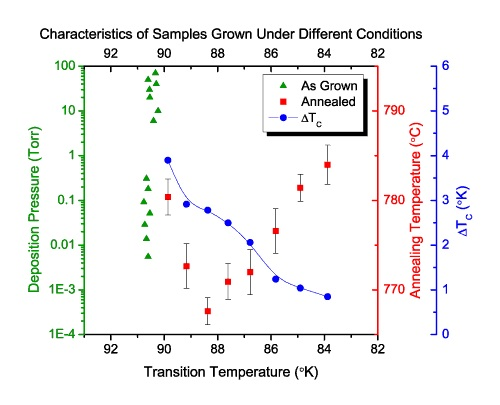
\includegraphics[width=\linewidth]{origin.jpg}
\caption{An example of single width figure
Solid lines show flight lines. K-A, K-B and N-B were active vents during the survey.}
\label{fig:view}
\end{figure}

Papers must highlight the impact and significance of the work for a materials readership to establish the suitability of the article for Algerian Journal of Advanced Materials. Papers that report incremental or derivative research should be directed to a more specialized journal.

\section{Equations}

Number all equations by enclosing in parentheses, and place the equation number to end at the light-hand margin. Equation numbers must be sequential. You can use sub numbering for equation numbers, if necessary. Make equations clear and legible, centered, with a space above and below. Place each equation on a separate line. Equations should be the same point size as the text. Please follow the standard style when writing equations: italics for variables, bold face for vectors, etc. Width of equation is within the column width. When you write long equations, you may think it is better to write equations in full width. In such a case, you can change the page style from a two column page to a full-width single column page.

\begin{equation}
\label{eq:emc}
e = mc^2
\end{equation}

\section{Tables}
Full papers contain original scientific work that has not been published previously. However, work that has appeared in print in a short form such as a communication is  acceptable. Please note that the Society strongly discourages the fragmentation of a substantial body of work into a number of short publications. Full papers contain original scientific work that has not been published previously. However, work that has appeared in print in a short form such as a communication is  acceptable. Please note that the Society strongly discourages the fragmentation of a substantial body of work into a number of short publications.

\begin{table}[h]
\centering
\begin{tabular}{c| c c}
%%\hline
\textbf{values} & \textbf{results 1} & \textbf{results 2}\\
\hline
100 & 0.0003262 & 0.562 \\
200 & 0.0015681 & 0.910 \\
300 & 0.0009271 & 0.296 \\
%%\hline
\end{tabular}
\caption{Results of values tests}
\end{table}

\section{Conclusions}
\label{S:2}

Type the word "References" as a heading in bold. For each reference, a dangling indent with 4 or 6 mm is preferable rather than numbering. For a journal paper: Last name(s) and initial(s) of author(s), year of publication, title of paper, name of journal (preferably in italic), volume number (bold), inclusive page numbers with hyphen.

\section{Acknowledgements}
\label{S:3}

The authors would like to express a sincere gratitude to the AMRS Committee of the CIGM4 to prepare this instruction.

\begin{thebibliography}{30} % Bibliography - this is intentionally simple in this template

\bibitem1{Zhou, H., and McMechan, G. A., 1997, One-pass 3-D seismic extrapolation with the 45o wave-equation, \textit{Geophysics}, 62, 1817- 1824.}

\bibitem1{van der Sluis, A., and van der Vorst, H. A., 1987, Numerical solution of large, sparse linear algebraic systems arising from tomographic problems, \textit{ Seismic Tomography}, Nolet, G. ed., Reidel, Dordrecht, 49-83.}

\bibitem1{Alkalifah, T., Biondi, B., and Fomel, S., 1998., Time-domain processing in arbitrary inhomogeneous media, 68th Ann International Meeting, Soc. Expl. Geophys., Expanded Abstract, 1750-1753.}
\end{thebibliography}
 
\end{document}

%% End of file `ajam-template.tex'.
